\subsubsection{Giới thiệu bộ dữ liệu}
    \paragraph{Nguồn dữ liệu}
    \leavevmode

    Đây là dữ liệu lượt khám chữa bệnh tại các cơ sở y tế tỉnh Sóc Trăng (ST), nhóm tự thu thập từ cơ sở dữ liệu chuyên ngành y tế HOC tỉnh Sóc Trăng

    \paragraph{Mô tả dữ liệu}
    \leavevmode

    Mỗi dòng dữ liệu chứa thông tin số lượng lượt khám chữa bệnh mỗi ngày. Khoảng dữ liệu từ này 01/01/2021 đến ngày 21/06/2025.

    Ví dụ một phần dữ liệu:

    \begin{table}[htbp]
    \centering
    \caption{Một phần bảng dữ liệu Khám chữa bệnh ST}
    \label{tab:stat-yte-exp}
        \begin{tabular}{|l|r|r|r|r|r|}
        \hline
        NGAYVAO & SO\_LUONG & E11 & E11\_9 & I10 & ... \\
        \hline
        2022-01-01 & 1201 & 21 & 145 & 246 & ... \\
        \hline
        2022-01-02 & 819 & 37 & 74 & 122 & ... \\
        \hline
        2022-01-03 & 1651 & 42 & 147 & 291 & ... \\
        \hline
        2022-01-04 & 6268 & 369 & 186 & 1741 & ... \\
        \hline
        ... & ... & ... & ... & ... \\
        \hline
        \end{tabular}

    \end{table}

    Bộ dữ liệu có 1268 dòng, bao gồm 15 cột như sau:

    \begin{itemize}
        \item Kiểu dữ liệu: \textbf{Quantitative} 
        \begin{itemize}
            \item \textbf{Continuous}:
             \begin{enumerate}[resume]
                \item \textbf{NGAYVAO}: Ngày khám

                \item \textbf{SO\_LUONG}: Tổng số lượt khám

                \item \textbf{E11}: Lượt khám bị bệnh đái tháo đường không phụ thuộc insuline
                \item \textbf{E11\_9}:	Bệnh đái tháo đường không phụ thuộc insuline (Chưa có biến chứng)
                \item \textbf{I10}: Lượt khám bị bệnh lý tăng huyết áp
                \item \textbf{J01}: Lượt khám bị bệnh viêm xoang cấp
                \item \textbf{J02}: Lượt khám bị bệnh viêm họng cấp
                \item \textbf{J06\_9}: Lượt khám bị bệnh nhiễm trùng đường hô hấp trên cấp, không phân loại
                \item \textbf{K21}: Lượt khám bị bệnh trào ngược dạ dày - thực quản
                \item \textbf{K21\_0}: Lượt khám bị bệnh trào ngược dạ dày - thực quản với viêm thực quản
                \item \textbf{J20}: Lượt khám bị bệnh viêm phế quản cấp
                \item \textbf{M25\_5}: Lượt khám bị bệnh đau khớp
                \item \textbf{M54\_5}: Lượt khám bị bệnh đau cột sống thắt lưng
                \item \textbf{R10\_4}: Lượt khám bị bệnh đau bụng không xác định và đau bụng khác
            \end{enumerate}

        \end{itemize}

    \end{itemize}

\subsubsection{Phân tích dữ liệu}
    \paragraph{Thống kê dữ liệu}
        \leavevmode

    Bảng \ref{tab:stat-yte} thể hiện các thông số thống kê trên một số đặc trưng của bộ dữ liệu.

    \begin{table}[htbp]
    \centering
    \caption{ Thống kê dữ liệu một số đặc trưng dữ liệu Lượt khám chữa bệnh ST}
    \label{tab:stat-yte}
    \begin{tabular}{|l|l|l|l|l|l|}
    \hline
      & SO\_LUONG & E11 & E11\_9 & I10 & J01 \\
    \hline
    Mean & 5,637.0662 & 199.8052 & 223.5213 & 883.0639 & 75.2634 \\
    \hline
    Min & 293 & 0 & 1 & 17 & 0 \\
    \hline
    Q1 & 2,869 & 38 & 171 & 397 & 13 \\
    \hline
    Median & 6,572.5 & 239 & 209 & 1,014 & 92.5 \\
    \hline
    Q3 & 7,384.25 & 292.25 & 265 & 1,187.25 & 113 \\
    \hline
    Max & 11,929 & 644 & 686 & 2,362 & 174 \\
    \hline
    Mode & 6,623 & 28 & 195 & 1,066 & 5 \\
    \hline
    Var & 6,138,540.7312 & 17,225.6739 & 6,730.8812 & 192,124.2856 & 2,359.326 \\
    \hline
    SD & 2,477.6079 & 131.2466 & 82.0419 & 438.3198 & 48.5729 \\
    \hline
    CV & 0.4395 & 0.6569 & 0.367 & 0.4964 & 0.6454 \\
    \hline
    IQR & 4,515.25 & 254.25 & 94 & 790.25 & 100 \\
    \hline
    \end{tabular}

    \end{table}

    Từ đây, ta có thể rút ra một số nhận xét:

    \begin{itemize}
        \item SO\_LUONG: Trung bình là 5637 lượt, trung vị 6572.5 cao hơn cho thấy phân phối hơi lệch trái, tức là có nhiều cơ sở y tế có lượt khám cao. Tuy nhiên, độ lệch chuẩn khá lớn (2477.6) và IQR = 4515.25 phản ánh mức độ chênh lệch lớn giữa các địa phương. 
        
        \item E11: Trung bình 199.8 ca mỗi đơn vị, trung vị cao hơn một chút (239), nhưng mode lại khá thấp (28) cho thấy một số nơi có số ca rất ít. Độ lệch chuẩn cao, 131.25, cho thấy dữ liệu có biến thiên lớn.
        
        \item E11\_9: Trung bình là 223.52, median = 209, và mode = 195 cho thấy phân phối tập trung quanh trung bình. Độ lệch chuẩn ở mức trung bình (82.04), và CV thấp hơn (0.367), cho thấy bệnh này được thống kê khá ổn định và đồng đều giữa các đơn vị.
        
        \item I10: trung bình 883 lượt mỗi đơn vị. Trung vị (1014) cao hơn trung bình và mode là 1066 cho thấy phân phối hơi lệch trái. 
        
        \item J01: Trung bình 75.26 thấp. Trung vị = 92.5 và mode = 5 cho thấy phân phối lệch phải. Độ lệch chuẩn khá lớn so với trung bình (SD = 48.57, CV = 0.6454). 
    
    \end{itemize}

    \paragraph{Trực quan hóa dữ liệu}
    \leavevmode

    \begin{figure}[htp]
        \centering
        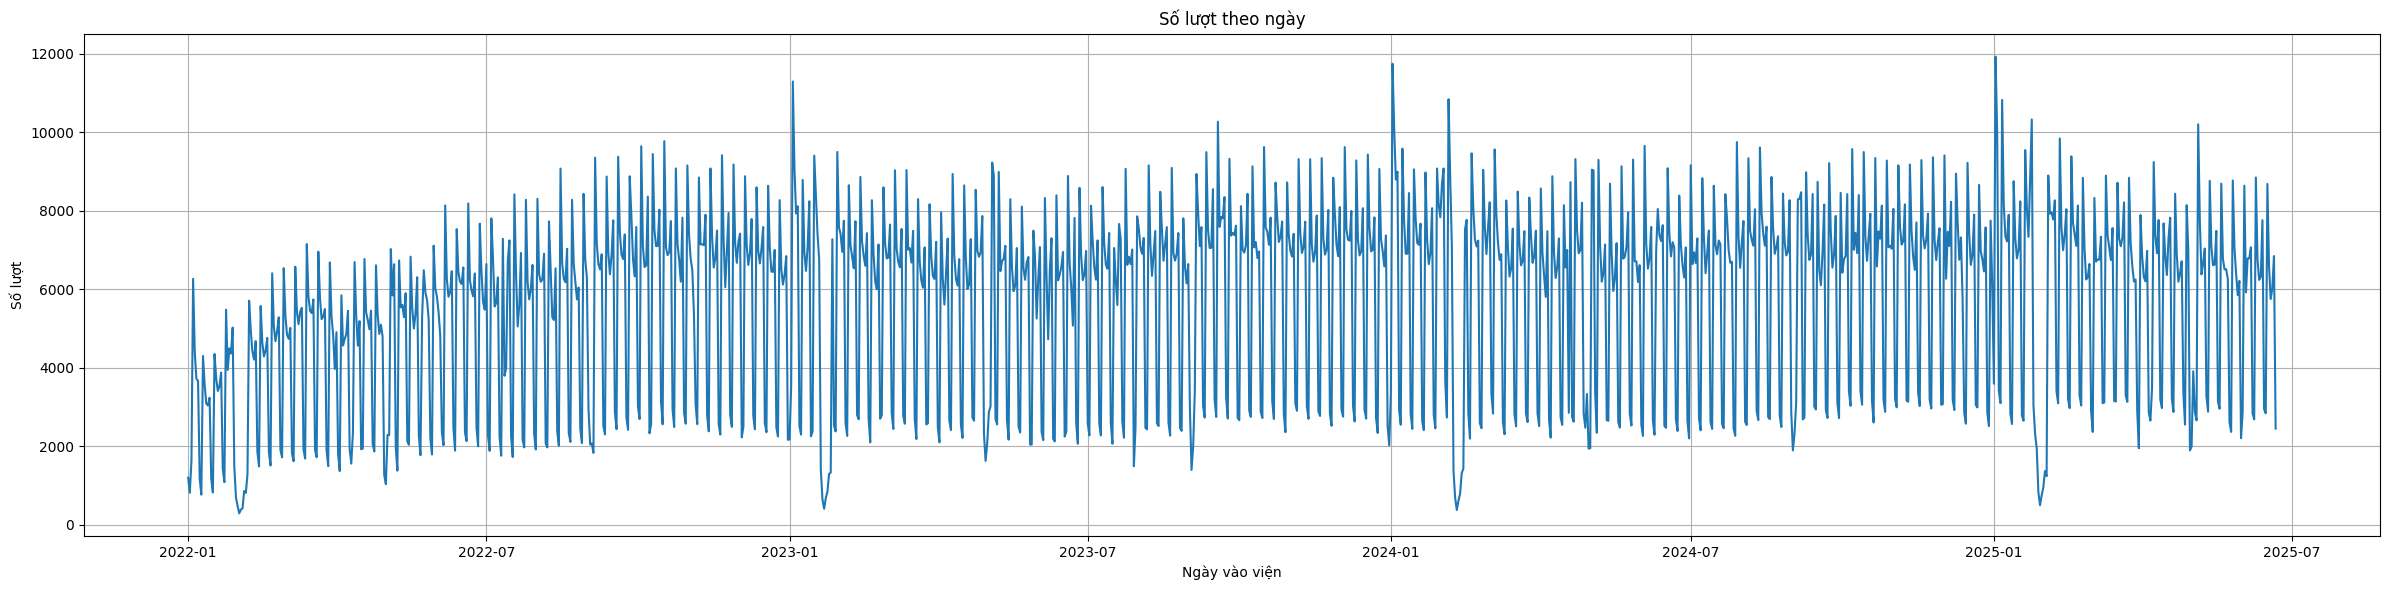
\includegraphics[width=0.90\textwidth]{images/TS_yte_tong.png}
        \caption{Số lượt khám ngày}
        \label{fig:TS_yte_tong}
    \end{figure}
    \FloatBarrier

    Biểu đồ \ref{fig:TS_yte_tong} cho thấy dao động mạnh giữa các ngày, khiến biểu đồ khó đọc. Ta có thể chuyển về trung bình lượt khám mỗi tuần để có biểu đồ cột dễ xem hơn.

    \begin{figure}[htp]
        \centering
        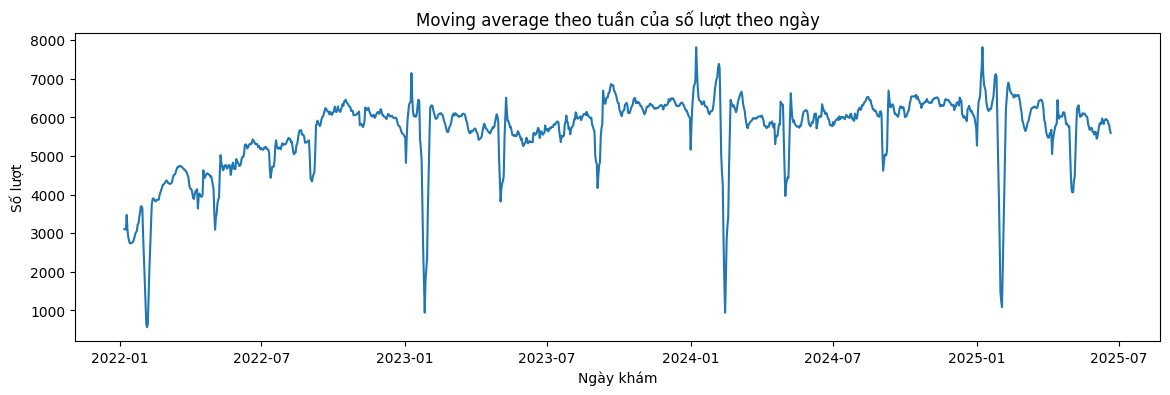
\includegraphics[width=0.90\textwidth]{images/TS_yte_tong_week.png}
        \caption{Số lượt khám trung bình tuần}
        \label{fig:TS_yte_tong_week}
    \end{figure}
    \FloatBarrier

    Biểu đồ \ref{fig:TS_yte_tong_week} cho thấy lượt khám trung bình theo tuần, đường lượt khám rõ ràng hơn so với ngày. Ta thấy biểu đồ có tính chu kỳ, mỗi năm số lượt khám ổn định khoản 6000 và có vài mốc giảm đột ngột.

    \begin{figure}[htp]
        \centering
        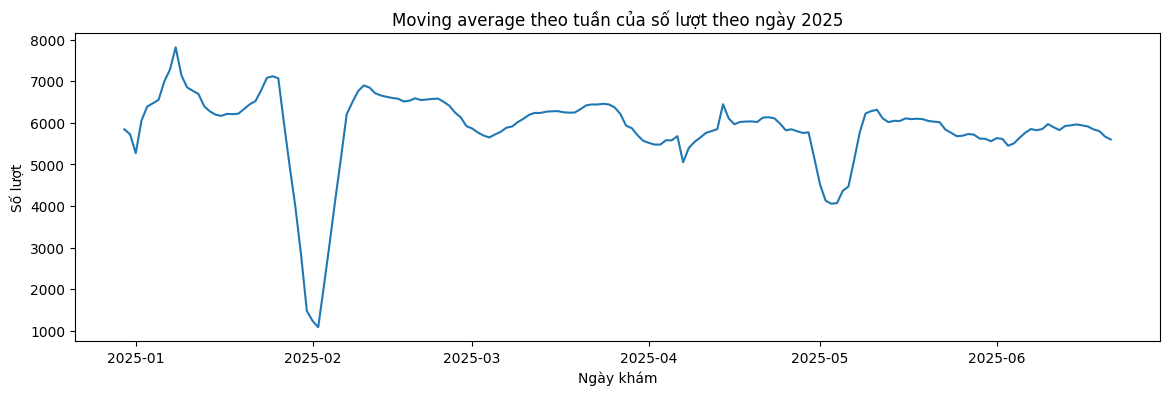
\includegraphics[width=0.80\textwidth]{images/TS_yte_tong_week2025.png}
        \caption{Số lượt khám trung bình tuần 2025}
        \label{fig:TS_yte_tong_week2025}
    \end{figure}
    \FloatBarrier

    \begin{figure}[htp]
        \centering
        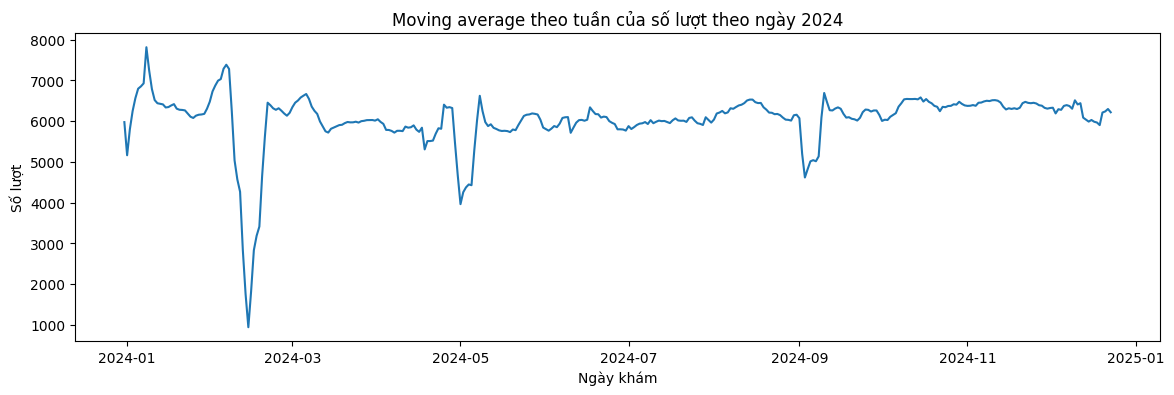
\includegraphics[width=0.80\textwidth]{images/TS_yte_tong_week2024.png}
        \caption{Số lượt khám trung bình tuần 2024}
        \label{fig:TS_yte_tong_week2024}
    \end{figure}
    \FloatBarrier

    \begin{figure}[htp]
        \centering
        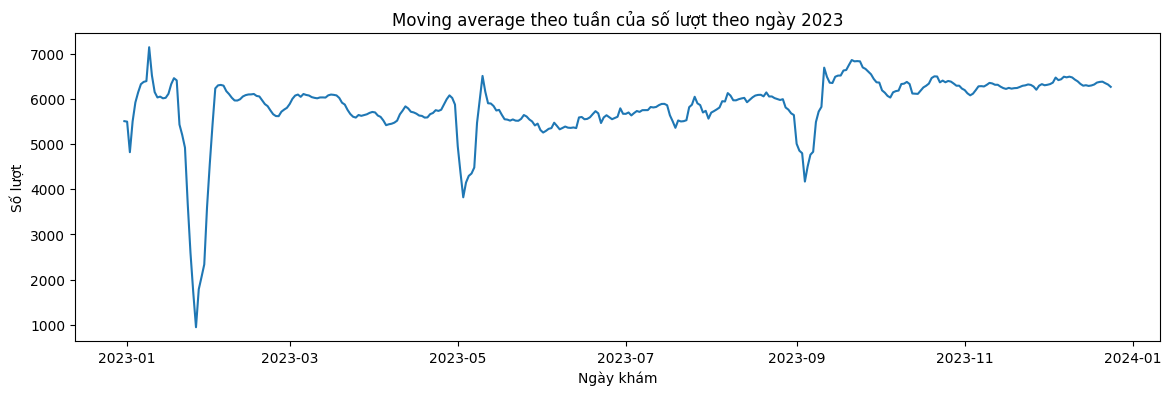
\includegraphics[width=0.80\textwidth]{images/TS_yte_tong_week2023.png}
        \caption{Số lượt khám trung bình tuần 2023}
        \label{fig:TS_yte_tong_week2023}
    \end{figure}
    \FloatBarrier

    Các biểu đồ \ref{fig:TS_yte_tong_week2025}, \ref{fig:TS_yte_tong_week2024}, \ref{fig:TS_yte_tong_week2023} phóng to số lượt khám trung bình tuần các năm 2025, 2024, 2023. Ta thấy được các đợt giảm đột ngột thường trùng vào dịp lễ có ngày nghỉ dài, cụ thể là Tết, 30/4, 2/9.

    \begin{figure}[htp]
        \centering
        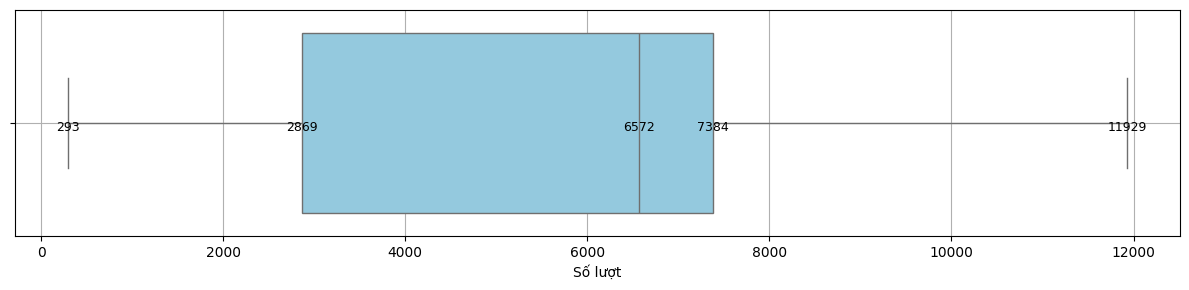
\includegraphics[width=0.80\textwidth]{images/TS_yte_tong_box.png}
        \caption{Số lượt khám}
        \label{fig:TS_yte_tong_box}
    \end{figure}
    \FloatBarrier

    Biểu đồ \ref{fig:TS_yte_tong_box} cho thấy số lượt khám mỗi ngày có sự dao động lớn, nhưng phần lớn tập trung trong khoảng từ gần 3000 đến hơn 7000 lượt. Trung vị đạt khoảng 6572 lượt, phản ánh mức độ hoạt động phổ biến của hệ thống y tế ở ngưỡng cao và ổn định. Tuy nhiên, vẫn tồn tại những ngày có số lượt tăng vọt gần 12000 hoặc giảm sâu xuống dưới 300. Những giá trị này có thể liên quan đến các dịp nghỉ lễ dài

    \begin{figure}[htp]
        \centering
        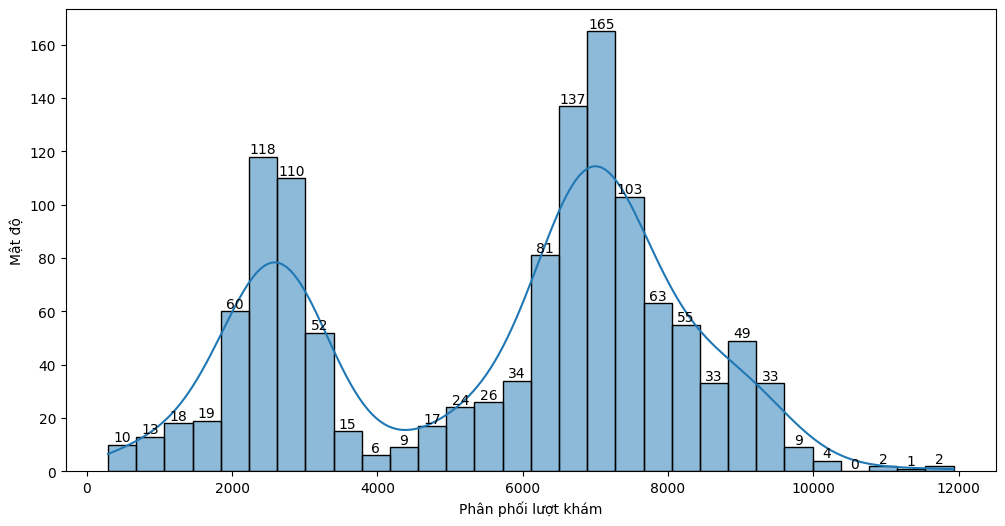
\includegraphics[width=0.80\textwidth]{images/TS_yte_tong_hist.png}
        \caption{Phân phối số lượt khám}
        \label{fig:TS_yte_tong_hist}
    \end{figure}
    \FloatBarrier

    Biểu đồ \ref{fig:TS_yte_tong_hist} thể hiện mật độ hai đỉnh, phân phối số lượt khám mỗi ngày không đồng nhất mà chia thành hai nhóm. Sự xuất hiện của hai đỉnh thể hiện đặc điểm hoạt động không liên tục.

    \begin{figure}[htp]
        \centering
        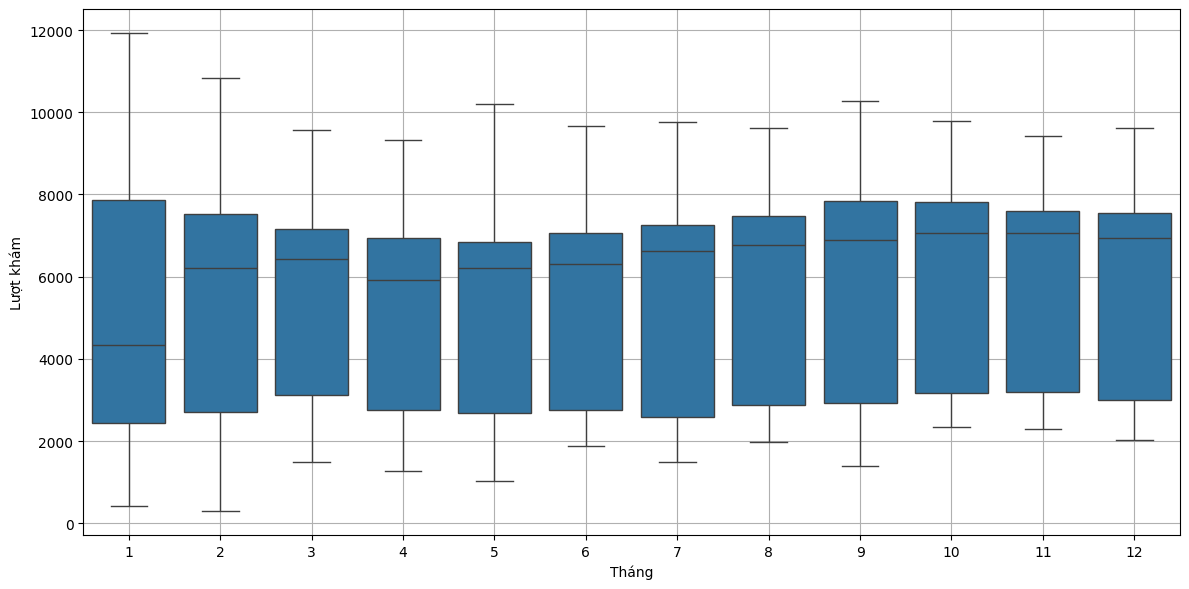
\includegraphics[width=0.80\textwidth]{images/TS_yte_tong_box_month.png}
        \caption{Số lượt khám qua các tháng}
        \label{fig:TS_yte_tong_box_month}
    \end{figure}
    \FloatBarrier

    Biểu đồ \ref{fig:TS_yte_tong_box_month}thể hiện phân bố số lượt khám bệnh theo từng tháng trong năm, phản ánh rõ sự biến động có tính mùa vụ. Tháng 1 có sự dao động mạnh nhất với nhiều giá trị thấp bất thường, có thể do tác động từ kỳ nghỉ Tết kéo dài. Các tháng còn lại ổn định hơn.

\subsubsection{Mô hình hóa dữ liệu}
    \paragraph{Cấu hình cài đặt} 
    \leavevmode

    Các mô hình sử dụng:

    \begin{itemize}
        \item \textbf{Linear Regression}: 

            \begin{lstlisting}[language=Python]
                LinearRegression()
            \end{lstlisting}

        \item \textbf{Random Forest Regressor}:

            \begin{lstlisting}[language=Python]
                RandomForestRegressor(
                    n_estimators=n_estimators, 
                    max_depth=max_depth, 
                    min_samples_leaf=min_samples_leaf
                )
            \end{lstlisting}

            khoảng hypertune tham số

            \begin{lstlisting}[language=Python]
                list_max_depth = [2, 3, 5, 10]
                list_n_estimators = [50, 100, 150, 200]
                list_min_samples_leaf = [1, 3, 5, 10]
            \end{lstlisting}.

        \item \textbf{XGBoost Classifier}:
            \begin{lstlisting}[language=Python]
                XGBRegressor(
                    n_estimators=n_estimators, 
                    max_depth=max_depth, 
                    reg_lambda=reg_lambda,
                    learning_rate=learning_rate,
                    reg_alpha=reg_alpha,
                )
            \end{lstlisting}

            khoảng hypertune tham số

            \begin{lstlisting}[language=Python]
                list_max_depth_xgb = [ 6, 7, 8]
                list_lambda = [0.5, 1, 2]
                list_learning_rate = [0.05, 0.1, 0.5]
                list_n_estimators_xgb  = [100, 150, 200]
                list_alpha = [0.5, 1]
            \end{lstlisting}.
        
    \end{itemize}

    Thuật toán data transform sử dụng: Standard Scaler.

    Chia tập dữ liệu huấn luyện: Train-Test: 80-20.

    \paragraph{Hồi quy số lượng khám chữa bệnh ngày 'SO\_LUONG'}
    \leavevmode

    Chuyển đặc trưng 'SO\_LUONG' về dạng sliding window để dự đoán hồi quy, thử nghiệm trên các khoảng: 30,90,180,365. Do số lượt khám có thể ảnh hưởng bởi mùa, điều kiện thời tiết,... nên chọn khoảng tháng, quý, nửa năm, năm.

    Kết quả:
    \begin{itemize}
        \item \textbf{Linear Regression}: 
        
            Mô hình tốt nhất:
            \begin{itemize}
                \item Khoảng sliding window: 90
            \end{itemize}

            \begin{table}[htbp]
            \centering
            \caption{Kết quả Linear Regression}
            \label{tab:yte-sl-lireg}
            \begin{tabular}{llrrr}
            \hline
             & Dataset & MAE & RMSE & MAPE \\
            \hline
            0 & Train & 516.283210 & 978.315505 & 15.271054 \\
            1 & Test & 634.900687 & 1128.755081 & 21.188820 \\
            \hline
            \end{tabular}
            \end{table}
  
            
            \FloatBarrier

            \begin{figure}[htp]
                \centering
                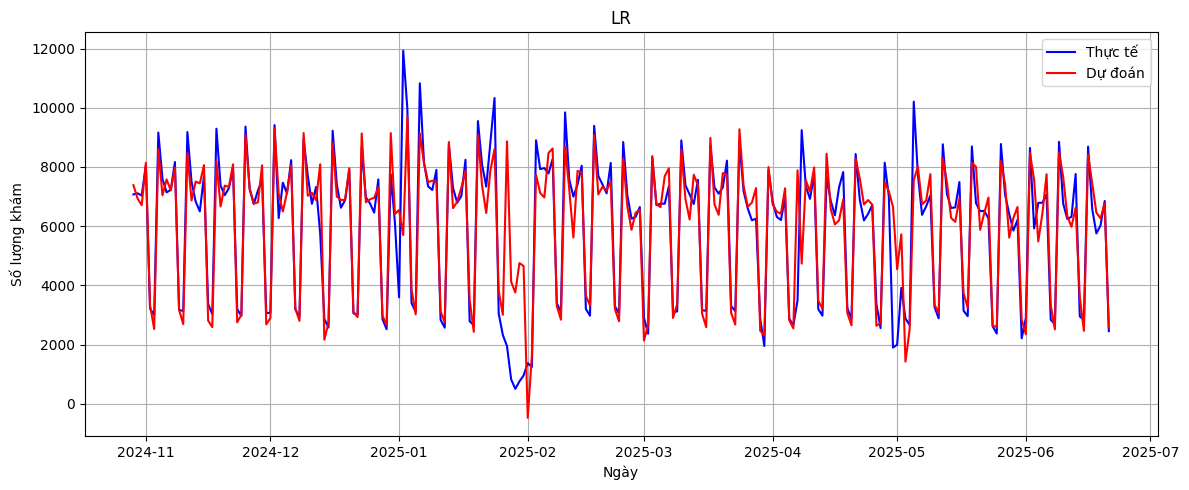
\includegraphics[width=0.90\textwidth]{images/TS_yte_pred_cmp_LR.png}
                \caption{Kết quả trên tập test Linear Regression}
                \label{fig:TS_yte_pred_cmp_LR}
            \end{figure}
        
            \FloatBarrier
            
        \item \textbf{Random Forest Regressor}:

            Mô hình tốt nhất:
            \begin{itemize}
                \item Khoảng sliding window: 30
                \item max\_depth: 10
                \item n\_estimators: 50
                \item min\_samples\_leaf: 3
            \end{itemize}

            \begin{table}[htbp]
                \centering
                \caption{Kết quả Random Forest Regressor}
                \label{tab:yte-sl-rf}
                \begin{tabular}{llrrr}
                \hline
                 & Dataset & MAE & RMSE & MAPE \\
                \hline
                0 & Train & 262.970338 & 520.311427 & 7.967650 \\
                1 & Test & 543.096956 & 1090.594231 & 17.977288 \\
                \hline
                \end{tabular}
            \end{table}
            
            \FloatBarrier

            \begin{figure}[htp]
                \centering
                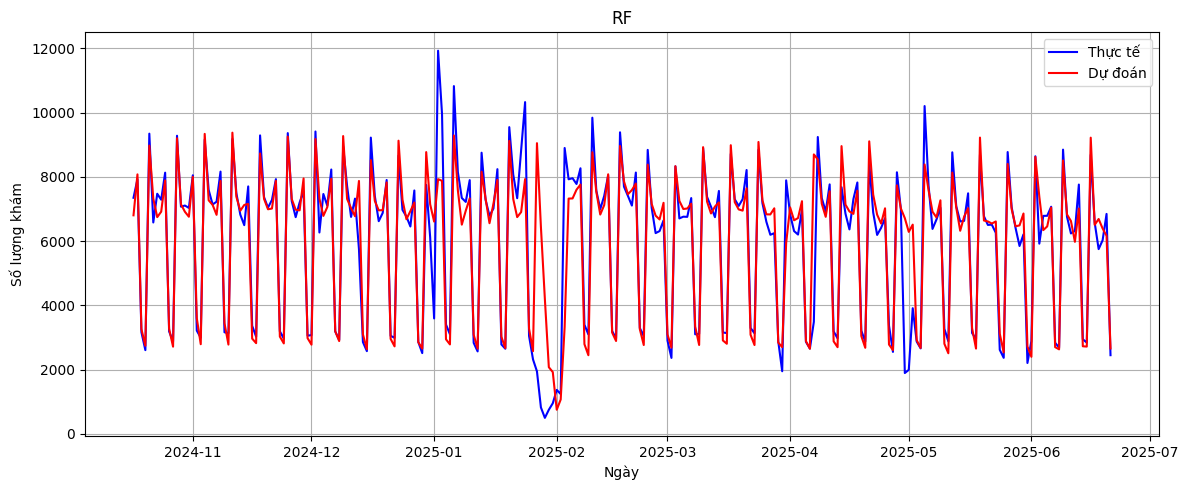
\includegraphics[width=0.90\textwidth]{images/TS_yte_pred_cmp_RF.png}
                \caption{Kết quả trên tập test RF Regressor}
                \label{fig:TS_yte_pred_cmp_RF}
            \end{figure}
            \FloatBarrier

        \item \textbf{XGBoost Regressor}:
        
            Mô hình tốt nhất:
            \begin{itemize}
                \item Khoảng sliding window: 90
                \item max\_depth: 8
                \item n\_estimators: 100
                \item reg\_lambda: 1
                \item reg\_alpha: 0.5
                \item learning\_rate: 0.5
            \end{itemize}

            \begin{table}[htbp]
                \centering
                \caption{Kết quả XGBoost Regressor}
                \label{tab:yte-sl-xgb}
                \begin{tabular}{llrrr}
                \hline
                 & Dataset & MAE & RMSE & MAPE \\
                \hline
                0 & Train & 31.960930 & 52.874545 & 0.864103 \\
                1 & Test & 590.553101 & 989.477861 & 14.796663 \\
                \hline
                \end{tabular}
            \end{table}

            \FloatBarrier

            \begin{figure}[htp]
                \centering
                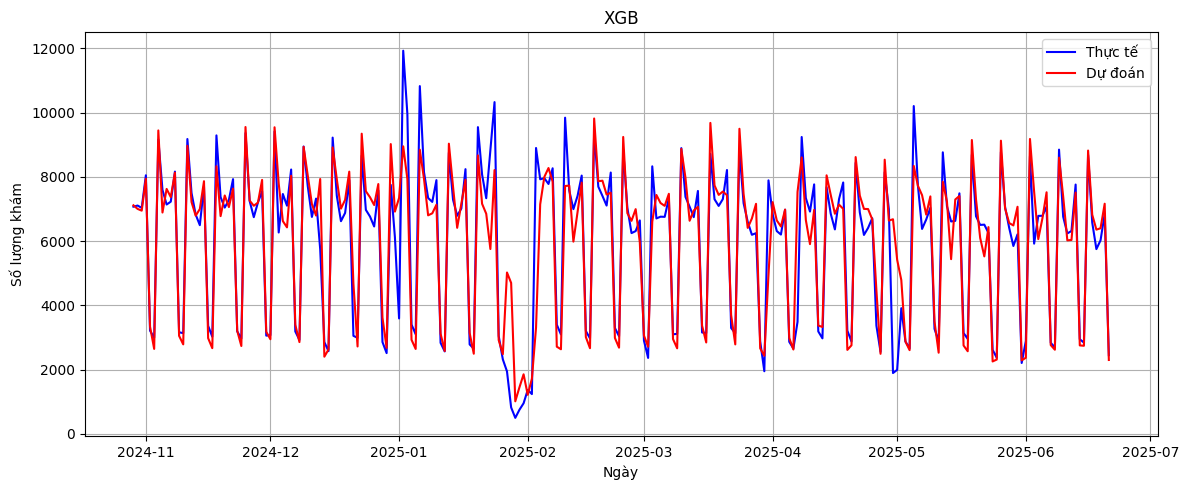
\includegraphics[width=0.90\textwidth]{images/TS_yte_pred_cmp_XGB.png}
                \caption{Kết quả trên tập test XGB Regressor}
                \label{fig:TS_yte_pred_cmp_XGB}
            \end{figure}
            \FloatBarrier
    \end{itemize}

    So sách các mô hình:

    \begin{table}[htbp]
        \centering
        \caption{So sánh kết quả các mô hình}
        \label{tab:yte-sl-compare}
        \begin{tabular}{|l|c|c|c|}
        \hline
        Model & MAE & RMSE & MAPE \\
        \hline
        Linear Regression & 634.900687 & 1128.755081 & 21.188820 \\
        \hline
        Random Forest & 543.096956 & 1090.594231 & 17.977288 \\
        \hline
        XGBoost & 590.553101 & 989.477861 & 14.796663 \\
        \hline
        \end{tabular}
    \end{table}

    \FloatBarrier

    Trong ba mô hình được đánh giá, Linear Regression cho thấy hiệu suất kém nhất với các sai số khá lớn trên tập kiểm tra (MAE = 634.90, RMSE = 1128.76, MAPE = 21.19\%), cho thấy mô hình tuyến tính đơn giản này không đủ khả năng nắm bắt các mối quan hệ phức tạp trong dữ liệu chuỗi thời gian. Random Forest Regressor cải thiện đáng kể độ chính xác so với Linear Regression, đặc biệt là ở chỉ số MAE và MAPE (lần lượt là 543.10 và 17.98\%). XGBoost Regressor là mô hình cho kết quả tốt nhất về tổng thể, với RMSE thấp nhất (989.48) và MAPE nhỏ nhất (14.80\%), mặc dù MAE cao hơn một chút so với Random Forest. Ở cả 3 mô hình (bảng \ref{tab:yte-sl-lireg}, \ref{tab:yte-sl-rf}, \ref{tab:yte-sl-xgb}), chỉ số lỗi train thấp nhưng test cao, có thể thấy các mô hình đang bị overfit.

\subsubsection{Kết luận}
    Trong phần này, nhóm đã tiến hành phân tích và xây dựng mô hình hồi quy dự đoán số lượt khám chữa bệnh các cơ sở y tế tỉnh Sóc Trăng. Kết quả thử nghiệm cho thấy Linear Regression có sai số cao và không phù hợp với dữ liệu chuỗi thời gian. Random Forest cải thiện độ chính xác đáng kể, trong khi XGBoost Regressor đạt hiệu suất tốt nhất với sai số thấp nhất. Tuy nhiên, cả ba mô hình đều cho thấy dấu hiệu overfitting, với sai số tập huấn luyện thấp hơn rõ rệt so với tập test. Nhóm nhận thấy cần cải thiện thêm về đặc trưng đầu vào và kỹ thuật regularization.